%%%%%%%%%%%%%%%%%%%%%%%%%%%%%%%%%%%%%%%%%%%%%%%%%%%%%%
%%%%%%%%%%%%%%%%%%%%%%%%%%%%%%%%%%%%%%%%%%%%%%%%%%%%%%%%%%%%%%%%%%%%
\def\scl{1}%scaling factor of the picture
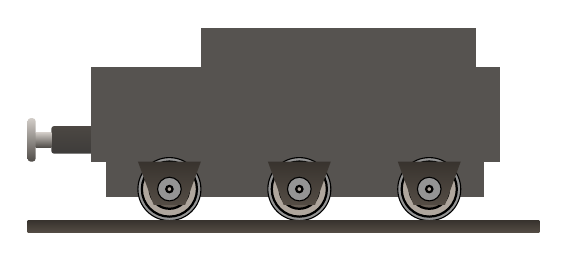
\begin{tikzpicture}[
  scale=\scl,
  tender/.style={gray!70!brown!20!black!75!},
  ]
%
%     TENDER
%
  \begin{scope}[xshift=0 cm,yshift=0 cm]

 % BUTOIR gauche
\def\hauteur{0.2}%
  \shade[bottom color=brown!10!gray!30!black!90!, top color=brown!20!gray!40!black!90!,rounded corners=1pt]
 (1.85, 0.9 + \hauteur) rectangle (0.3, 1.25 + \hauteur);
  \shade[bottom color=brown!10!gray!60!black, top color=brown!20!gray!40!]
 (0.3, 0.98 + \hauteur) rectangle (0.1, 1.17 + \hauteur);
  \shade[bottom color=brown!10!gray!60!black, top color=brown!20!gray!40!,rounded corners=1pt]
 (0, 0.8 + \hauteur) rectangle (0.1, 1.35 + \hauteur);

 % CORPS

    \fill[tender] (0.8, 1.0) rectangle (6.0, 2.2); % milieux

    \fill[tender] (2.2, 2.2) rectangle (5.7, 2.7); % haut

\def\hauteur{0.65} % hauteur des roues

    \fill[tender] (1.0,  \hauteur - 0.1) rectangle (5.8, 1.0); % bas

%  ROUES
  \foreach \x in {0, 1,..., 2}
 { \fill[black!20!gray!70!,draw=black,thin] (1.8 +\x * 1.65, \hauteur) circle (0.4 cm);
  \fill[brown!20!gray!70!,draw=black,thick] (1.8 +\x * 1.65, \hauteur) circle (0.35 cm);
  \fill[brown!20!black!70!,draw=black,thick] (1.8 +\x * 1.65, \hauteur) circle (0.25 cm); }

 % ESSIEUX
  \foreach \x in {0, 1,..., 2}
 { \shade[bottom color=brown!20!gray!60!black, top color=brown!20!gray!40!black]
 (1.6 +\x * 1.65, \hauteur -0.2) -- (2.0 +\x * 1.65, \hauteur -0.2) -- (2.2 +\x * 1.65, 1.0) -- (1.4 +\x * 1.65, 1.0) -- cycle;
  \fill[black!20!gray!70!,draw=black,thin] (1.8 +\x * 1.65, \hauteur) circle (0.15 cm);
  \fill[brown!20!gray!70!,draw=black,thick] (1.8 +\x * 1.65, \hauteur) circle (0.04 cm); }

  % RAIL
  \shade[bottom color=brown!20!gray!60!black, top color=brown!20!gray!40!black]
 (0, 0.25) rectangle (6.5, 0.1);

  \end{scope}
%
%
\end{tikzpicture}
%
